\documentclass[a4paper]{article}
\usepackage[]{graphicx}\usepackage[]{color}
% maxwidth is the original width if it is less than linewidth
% otherwise use linewidth (to make sure the graphics do not exceed the margin)
\makeatletter
\def\maxwidth{ %
  \ifdim\Gin@nat@width>\linewidth
    \linewidth
  \else
    \Gin@nat@width
  \fi
}
\makeatother

\definecolor{fgcolor}{rgb}{0.345, 0.345, 0.345}
\newcommand{\hlnum}[1]{\textcolor[rgb]{0.686,0.059,0.569}{#1}}%
\newcommand{\hlstr}[1]{\textcolor[rgb]{0.192,0.494,0.8}{#1}}%
\newcommand{\hlcom}[1]{\textcolor[rgb]{0.678,0.584,0.686}{\textit{#1}}}%
\newcommand{\hlopt}[1]{\textcolor[rgb]{0,0,0}{#1}}%
\newcommand{\hlstd}[1]{\textcolor[rgb]{0.345,0.345,0.345}{#1}}%
\newcommand{\hlkwa}[1]{\textcolor[rgb]{0.161,0.373,0.58}{\textbf{#1}}}%
\newcommand{\hlkwb}[1]{\textcolor[rgb]{0.69,0.353,0.396}{#1}}%
\newcommand{\hlkwc}[1]{\textcolor[rgb]{0.333,0.667,0.333}{#1}}%
\newcommand{\hlkwd}[1]{\textcolor[rgb]{0.737,0.353,0.396}{\textbf{#1}}}%
\let\hlipl\hlkwb

\usepackage{framed}
\makeatletter
\newenvironment{kframe}{%
 \def\at@end@of@kframe{}%
 \ifinner\ifhmode%
  \def\at@end@of@kframe{\end{minipage}}%
  \begin{minipage}{\columnwidth}%
 \fi\fi%
 \def\FrameCommand##1{\hskip\@totalleftmargin \hskip-\fboxsep
 \colorbox{shadecolor}{##1}\hskip-\fboxsep
     % There is no \\@totalrightmargin, so:
     \hskip-\linewidth \hskip-\@totalleftmargin \hskip\columnwidth}%
 \MakeFramed {\advance\hsize-\width
   \@totalleftmargin\z@ \linewidth\hsize
   \@setminipage}}%
 {\par\unskip\endMakeFramed%
 \at@end@of@kframe}
\makeatother

\definecolor{shadecolor}{rgb}{.97, .97, .97}
\definecolor{messagecolor}{rgb}{0, 0, 0}
\definecolor{warningcolor}{rgb}{1, 0, 1}
\definecolor{errorcolor}{rgb}{1, 0, 0}
\newenvironment{knitrout}{}{} % an empty environment to be redefined in TeX

\usepackage{alltt}
\newcommand{\SweaveOpts}[1]{}  % do not interfere with LaTeX
\newcommand{\SweaveInput}[1]{} % because they are not real TeX commands
\newcommand{\Sexpr}[1]{}       % will only be parsed by R




\usepackage[utf8]{inputenc}
%\usepackage[ngerman]{babel}
\usepackage{a4wide,paralist}
\usepackage{amsmath, amssymb, xfrac, amsthm}
\usepackage{dsfont}
\usepackage[usenames,dvipsnames]{xcolor}
\usepackage{amsfonts}
\usepackage{graphicx}
\usepackage{caption}
\usepackage{subcaption}
\usepackage{framed}
\usepackage{multirow}
\usepackage{bytefield}
\usepackage{csquotes}
\usepackage[breakable, theorems, skins]{tcolorbox}
\usepackage{hyperref}
\usepackage{cancel}
\usepackage{bm}


\input{../../style/common}

\tcbset{enhanced}

\DeclareRobustCommand{\mybox}[2][gray!20]{%
	\iffalse
	\begin{tcolorbox}[   %% Adjust the following parameters at will.
		breakable,
		left=0pt,
		right=0pt,
		top=0pt,
		bottom=0pt,
		colback=#1,
		colframe=#1,
		width=\dimexpr\linewidth\relax,
		enlarge left by=0mm,
		boxsep=5pt,
		arc=0pt,outer arc=0pt,
		]
		#2
	\end{tcolorbox}
	\fi
}

\DeclareRobustCommand{\myboxshow}[2][gray!20]{%
%	\iffalse
	\begin{tcolorbox}[   %% Adjust the following parameters at will.
		breakable,
		left=0pt,
		right=0pt,
		top=0pt,
		bottom=0pt,
		colback=#1,
		colframe=#1,
		width=\dimexpr\linewidth\relax,
		enlarge left by=0mm,
		boxsep=5pt,
		arc=0pt,outer arc=0pt,
		]
		#2
	\end{tcolorbox}
%	\fi
}


%exercise numbering
\renewcommand{\theenumi}{(\alph{enumi})}
\renewcommand{\theenumii}{\roman{enumii}}
\renewcommand\labelenumi{\theenumi}


\font \sfbold=cmssbx10

\setlength{\oddsidemargin}{0cm} \setlength{\textwidth}{16cm}


\sloppy
\parindent0em
\parskip0.5em
\topmargin-2.3 cm
\textheight25cm
\textwidth17.5cm
\oddsidemargin-0.8cm
\pagestyle{empty}

\newcommand{\kopf}[1] {
\hrule
\vspace{.15cm}
\begin{minipage}{\textwidth}
%akwardly i had to put \" here to make it compile correctly
	{\sf\bf Introduction to Machine Learning \hfill Exercise sheet #1\\
	 \url{https://introduction-to-machine-learning.netlify.app/} \hfill WiSe 2020/2021}
\end{minipage}
\vspace{.05cm}
\hrule
\vspace{1cm}}

\newenvironment{allgemein}
	{\noindent}{\vspace{1cm}}

\newcounter{aufg}
\newenvironment{aufgabe}
	{\refstepcounter{aufg}\textbf{Exercise \arabic{aufg}:}\\ \noindent}
	{\vspace{0.5cm}}

\newcounter{loes}
\newenvironment{loesung}
	{\refstepcounter{loes}\textbf{Solution \arabic{loes}:}\\\noindent}
	{\bigskip}
	
\newenvironment{bonusaufgabe}
	{\refstepcounter{aufg}\textbf{Exercise \arabic{aufg}*\footnote{This
	is a bonus exercise.}:}\\ \noindent}
	{\vspace{0.5cm}}

\newenvironment{bonusloesung}
	{\refstepcounter{loes}\textbf{Solution \arabic{loes}*:}\\\noindent}
	{\bigskip}



\begin{document}
% !Rnw weave = knitr



\input{../../latex-math/basic-math.tex}
\input{../../latex-math/basic-ml.tex}

\kopf{1}

\loesung{

\begin{enumerate}
  \item[a)] multiclass classification (plate digits) (supervised learning)
  \item[b)] binary classification (supervised)
  \item[c)] outlier detection ((un)supervised)
  \item[d)] frequent pattern mining (unsupervised)
  \item[e)] classification (supervised) / clustering (unsupervised)
  \item[f)] classification (supervised)
  \item[g)] clustering / assocation rules (unsupervised)
  \item[h)] not a machine learning task
  \item[i)] not a machine learning task
\end{enumerate}
}

\dlz
\loesung{




\begin{enumerate}
\item[a)] We use the least squares-estimator introduced in the lecture:
\lz
$\hat{\beta} = (X^TX)^{-1}X^Ty$  with \\ $ X = \begin{bmatrix}
1 & x_{1,1} & x_{1,2} & ... & x_{1,m} \\
1 & x_{2,1} & x_{2,2} & ... & x_{2,m} \\
\vdots & \vdots & \vdots & ... & \vdots \\
1 & x_{n,1} & x_{n,2} & ... & x_{n,m} \\
\end{bmatrix}
\lz
$  \\
$ x =  \begin{bmatrix}
0.56  \\
0.22  \\
1.7  \\
0.63  \\
0.36  \\
1.2  \\
\end{bmatrix}, X =  \begin{bmatrix}
1 & 0.56  \\
1 & 0.22  \\
1 & 1.7  \\
1 & 0.63  \\
1 & 0.36  \\
1 & 1.2  \\
\end{bmatrix}
$
and
 $
y =  \begin{bmatrix}
160  \\
150  \\
175  \\
185  \\
165  \\
170  \\
\end{bmatrix}
$

Then \begin{align*}
\hat{\beta} &= (X^TX)^{-1}X^Ty \\ &= \left(
\begin{bmatrix}
1 & 1 & 1 & ... & 1  \\
x_{1,1} & x_{2,1} & x_{3,1} & ... & x_{n,1} \\
\vdots & \vdots & \vdots & ... & \vdots \\
x_{1,m} & x_{2,m} & x_{3,m} & ... & x_{n,m} \\
\end{bmatrix}
\begin{bmatrix}
1 & x_{1,1} & x_{1,2} & ... & x_{1,m} \\
1 & x_{2,1} & x_{2,2} & ... & x_{2,m} \\
\vdots & \vdots & \vdots & ... & \vdots \\
1 & x_{n,1} & x_{n,2} & ... & x_{n,m} \\
\end{bmatrix} \right)^{-1}\begin{bmatrix}
1 & 1 & 1 & ... 1  \\
x_{1,1} & x_{2,1} & x_{3,1} & ... & x_{n,1} \\
\vdots & \vdots & \vdots & ... & \vdots \\
x_{1,m} & x_{2,m} & x_{3,m} & ... & x_{n,m} \\
\end{bmatrix}
\begin{bmatrix}
160  \\
150  \\
175  \\
185  \\
165  \\
170  \\
\end{bmatrix} \\ &= \left(
\begin{bmatrix}
1 & 1 & 1 & 1 & 1 & 1 \\
0.56 & 0.22 & 1.7 & 0.63 & 0.36 &  1.2   \\
\end{bmatrix}
\begin{bmatrix}
1 & 0.56  \\
1 & 0.22  \\
1 & 1.7  \\
1 & 0.63  \\
1 & 0.36  \\
1 & 1.2  \\
\end{bmatrix} \right)^{-1}
\begin{bmatrix}
1 & 1 & 1 & 1 & 1 & 1 \\
0.56 & 0.22 & 1.7 & 0.63 & 0.36 &  1.2   \\
\end{bmatrix}
\begin{bmatrix}
160  \\
150  \\
175  \\
185  \\
165  \\
170  \\
\end{bmatrix} \\ &=
\begin{bmatrix}
6 & 4.67  \\
4.67 & 5.2185   \\
\end{bmatrix}^{-1}
\begin{bmatrix}
1 & 1 & 1 & 1 & 1 & 1 \\
0.56 & 0.22 & 1.7 & 0.63 & 0.36 &  1.2   \\
\end{bmatrix}
\begin{bmatrix}
160  \\
150  \\
175  \\
185  \\
165  \\
170  \\
\end{bmatrix} \\ &=
 \begin{bmatrix}
0.5491944 & -0.4914703  \\
-0.4914703  & 0.6314394   \\
\end{bmatrix}
\begin{bmatrix}
1 & 1 & 1 & 1 & 1 & 1 \\
0.56 & 0.22 & 1.7 & 0.63 & 0.36 &  1.2   \\
\end{bmatrix}
\begin{bmatrix}
160  \\
150  \\
175  \\
185  \\
165  \\
170  \\
\end{bmatrix} \\
&= \begin{bmatrix}
0.2739710 & 0.4410709 & -0.2863051  & 0.23956809 & 0.3722651 & -0.04056998 \\
-0.1378643 & -0.3525536 & 0.5819766 & -0.09366351 & -0.2641521 & 0.26625693 \\
\end{bmatrix}
\begin{bmatrix}
160  \\
150  \\
175  \\
185  \\
165  \\
170  \\
\end{bmatrix} \\
&= \begin{bmatrix}
158.73954  \\
11.25541  \\
\end{bmatrix}
\end{align*}


Hence the linear model $\hat{y} = \hat{\beta}_0 + \hat{\beta}_1 x = 158.73954 + 11.25541 x$

\begin{knitrout}
\definecolor{shadecolor}{rgb}{0.969, 0.969, 0.969}\color{fgcolor}\begin{kframe}
\begin{alltt}
\hlstd{x} \hlkwb{=} \hlkwd{c}\hlstd{(}\hlnum{0.56}\hlstd{,} \hlnum{0.22}\hlstd{,} \hlnum{1.7}\hlstd{,} \hlnum{0.63}\hlstd{,} \hlnum{0.36}\hlstd{,}\hlnum{1.2}\hlstd{)}
\hlstd{y} \hlkwb{=} \hlkwd{c}\hlstd{(}\hlnum{160}\hlstd{,}\hlnum{150}\hlstd{,}\hlnum{175}\hlstd{,}\hlnum{185}\hlstd{,}\hlnum{165}\hlstd{,}\hlnum{170}\hlstd{)}

\hlstd{X} \hlkwb{<-} \hlkwd{sapply}\hlstd{(}\hlnum{0}\hlopt{:}\hlnum{1}\hlstd{,} \hlkwa{function}\hlstd{(}\hlkwc{k}\hlstd{) x}\hlopt{^}\hlstd{k)}
\hlkwd{solve}\hlstd{(}\hlkwd{t}\hlstd{(X)} \hlopt \hlstd{X)} \hlopt \hlkwd{t}\hlstd{(X)} \hlopt \hlstd{y}
\end{alltt}
\begin{verbatim}
##           [,1]
## [1,] 158.73954
## [2,]  11.25541
\end{verbatim}
\end{kframe}
\end{knitrout}

\begin{knitrout}
\definecolor{shadecolor}{rgb}{0.969, 0.969, 0.969}\color{fgcolor}

{\centering 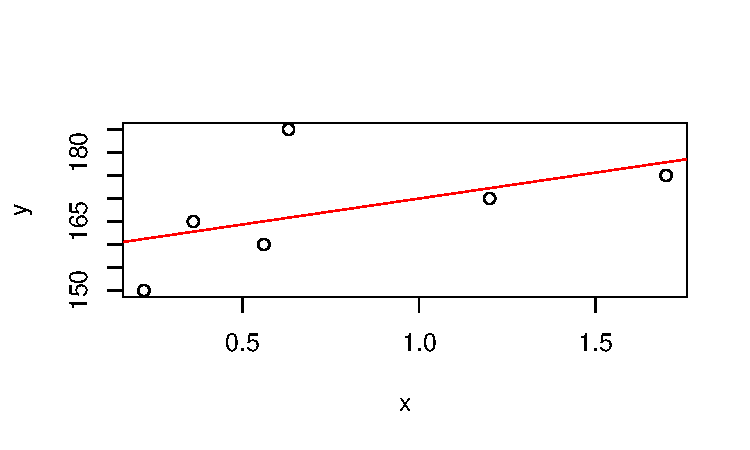
\includegraphics[width=\maxwidth]{figure/unnamed-chunk-6-1} 

}


\end{knitrout}


\item[b)]
Here  $
X =  \begin{bmatrix}
1 & 0.56 & 0.3136 \\
1 & 0.22 & 0.0484 \\
1 & 1.7 & 2.89 \\
1 & 0.63 & 0.3969 \\
1 & 0.36 & 0.1296 \\
1 & 1.2  & 1.44\\
\end{bmatrix}
$
 and $\hat{\beta} =  \begin{bmatrix}
143.51682 \\
57.59155 \\
-23.96347 \\
\end{bmatrix} $

\begin{knitrout}
\definecolor{shadecolor}{rgb}{0.969, 0.969, 0.969}\color{fgcolor}\begin{kframe}
\begin{alltt}
\hlstd{x} \hlkwb{=} \hlkwd{c}\hlstd{(}\hlnum{0.56}\hlstd{,} \hlnum{0.22}\hlstd{,} \hlnum{1.7}\hlstd{,} \hlnum{0.63}\hlstd{,} \hlnum{0.36}\hlstd{,}\hlnum{1.2}\hlstd{)}
\hlstd{y} \hlkwb{=} \hlkwd{c}\hlstd{(}\hlnum{160}\hlstd{,}\hlnum{150}\hlstd{,}\hlnum{175}\hlstd{,}\hlnum{185}\hlstd{,}\hlnum{165}\hlstd{,}\hlnum{170}\hlstd{)}

\hlstd{X} \hlkwb{<-} \hlkwd{sapply}\hlstd{(}\hlnum{0}\hlopt{:}\hlnum{2}\hlstd{,} \hlkwa{function}\hlstd{(}\hlkwc{k}\hlstd{) x}\hlopt{^}\hlstd{k)}
\hlkwd{solve}\hlstd{(}\hlkwd{t}\hlstd{(X)} \hlopt \hlstd{X)} \hlopt \hlkwd{t}\hlstd{(X)} \hlopt \hlstd{y}
\end{alltt}
\begin{verbatim}
##           [,1]
## [1,] 143.51681
## [2,]  57.59155
## [3,] -23.96347
\end{verbatim}
\end{kframe}
\end{knitrout}


\begin{knitrout}
\definecolor{shadecolor}{rgb}{0.969, 0.969, 0.969}\color{fgcolor}

{\centering 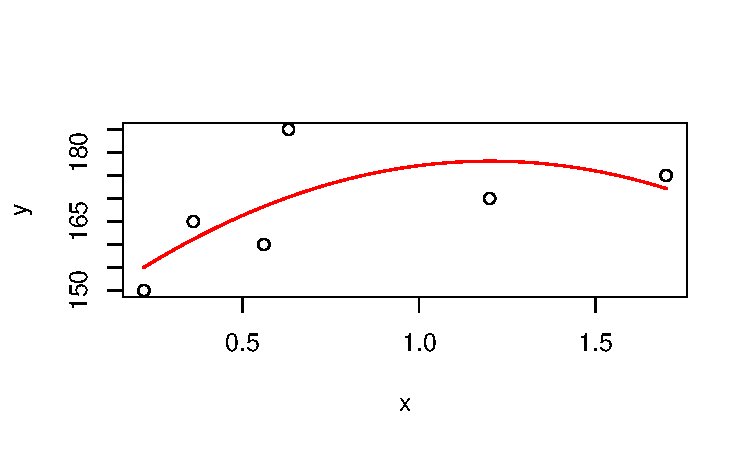
\includegraphics[width=\maxwidth]{figure/unnamed-chunk-8-1} 

}


\end{knitrout}


\end{enumerate}
}

\newpage

\dlz
\loesung{


\begin{enumerate}[a)]
  \item Supervised learning problem - the model will be learned from historical
  credit data for which payment history has been observed (knowing the ground
  truth is vital here since we need to evaluate our model's accuracy)
  \item Target variable: classes (default y/n), continuous credit
  scores, or class probabilities). Potential features: monthly income, current 
  level of indebtedness, past credit behavior, profession, residential 
  environment, age, number of kids etc. Labels: yes, since we have a supervised 
  learning problem.
  \item This is a classification problem - we want to assign our customers to
  classes \emph{default} and \emph{non-default}.
  \item (Primarily) learning to predict - we want to score future borrowers.
  \item $\Hspace = \{\pi: \Xspace \mapsto [0,1] ~|~ \pixt = s(\thetab^T \xv), \thetab \in \R^d\}$,
  where $s(z) = 1 / (1 + exp(-z))$ is the sigmoid function. Parameters to be
  learned: $\thetab$.
  \item We know that, in the optimum, (log-)likelihood is maximal. We can
  directly translate this into risk minimization by using the \emph{negative}
  log-likelihood as our empirical risk. We will just use the pointwise negative
  log-likelihood as our loss function: $$\Lpixyit = - \left(\yi \log \left(
  \pixit \right) + \left(1 - \yi \right) \left(\log \left(1 - \pixit \right) 
  \right) \right)$$ (the so-called \emph{Bernoulli loss}). The
  empirical risk is then the sum of point-wise losses: $$\risket = -\sumin \yi
  \log \left(\pixit \right) + \left(1 - \yi \right) \left(\log \left(1 - \pixit
  \right) \right)$$
  \item We can now solve this optimization problem via empirical risk
  minimization, which, in this case, is perfectly equivalent to ML estimation.
  Therefore, we set the first derivative of $\risket$ wrt $\thetab$ to 0 and
  solve for $\thetab$. However -- unlike linear regression -- this has no
  closed-form solution, so a numerical optimization procedure such as gradient
  descent is required.
\end{enumerate}
}
\end{document}
